\chapter{Proposed Approach}

\section{Overview}

Our method specifically focused on Source Identification and Integrity Verification. In the following, we will explain the theory behind our proposed approach, that is the main idea of why and how to use video file containers for Multimedia Forensics.

As mentioned in the previous chapters, file containers contain structured information about the video such as content-related metadata (acquisition time, modification time, place, etc.), number of tracks and signals (audio and video), and codec data (quantization tables, etc.) that is necessary to decode and present the signal. Since the file format standards leave room for freedom to the manufacturers about how the file container is composed, we can harness both its content and, mostly, its structure. The idea behind the use of file containers is that both the source device or the platform from which a video originates leave traces on its containers so that we can determine its history.

For Source Identification, we are in this scenario: given a query video we want to assess if it belongs to a class $C$ based on its file container, where for a class we mean a source of origin. Specifically, during this thesis, we have focused our study on video file generated from smartphones. In this case, we can imagine the possible classes as having a hierarchic structure; so a class could be seen a specific brand, a specific model of a certain brand, or a particular operating system on a certain brand of some brand of smartphones.

Basically, given a query video and a class $C$, we pose a binary question: does this query video belongs to the class $C$? To answer that question, we split the ground truth set of videos into two classes $X_{C}$ and $X_{\overline{C}}$, i.e. of videos belonging to class $C$ and not respectively.

To determine which of the two classes the query video belongs, we need a compatibility score. We create $\Omega$ that is the set of all the attributes $\omega$ of the atoms contained in each file containers of the ground truth media. We determine the discrimination power of each attributes $\omega$ for the class $C$,

$$  W_{C}(\omega) = \dfrac{\sum\limits_{i=1}^{N_{C}}\mid X_{i} \cap \omega \mid}{N_{C}} $$

with $X_{i} \in X_{C}$ and $N_{C}$ the number of videos of the ground truth that belongs to the class $C$.

Similarly, we compute the discrimination power of each attributes $\omega$ for the classe $\overline{C}$,

$$  W_{\overline{C}}(\omega) = \dfrac{\sum\limits_{i=1}^{N_{\overline{C}}}\mid X_{i} \cap \omega \mid}{N_{\overline{C}}} $$

with $X_{i} \in X_{\overline{C}}$ and $N_{\overline{C}}$ the number of videos of the ground truth that belongs to the class $\overline{C}$.

With the discrimination power, we can determine how important an attribute is for a particular class.

The procedure described above is what we refer to as the training phase. For the test phase, given a query video $X = \left\lbrace \omega_{1},...,\omega_{n} \right\lbrace $, we solve the two hypothesis test problem:

$$  H_{0}:X \in \overline{C} $$
$$  H_{1}:X \in C $$

Then we determine the likelihood of observing $\omega_{j} \in X, j = 1,...,t$ for each of the two classes.

$$ P(\omega_{j}\vert H_{0}) = \Omega_{\overline{C}}(\omega_{j}) $$
$$ P(\omega_{j}\vert H_{1}) = \Omega_{C}(\omega_{j}) $$ 

Supposing, that $\omega_{j}$ are independently distributed we can compute a likelihood

$$ L(X) = \dfrac{\prod\limits_{\omega_{j}} \Omega_{C}(\omega_{j} }{\Omega_{\overline{C}}(\omega_{j}} $$

to determine whether a query video $X$ to belong to the class $C$.

For Integrity Verification, the approach is simpler because we don't need to deal with classes. In this scenario, we have a query video $X$ that supposedly come from a certain device, and we want to assess if this supposition is correct or if the video has undergone some other processing step during its lifecycle. To do that, we create a reference video $Y$ with the device that supposedly is the source of the video $X$; to assess the integrity, we need to determine the compatibility of the file containers of the query video $X$ with the file container of the reference video $Y$. 

For each attribute of $Y$, we check their presence in the file containers of $X$; then we do the same operation in reverse, that is checking the presence of the attributes of $X$ in the file containers of $Y$. The results will be a percentage representing a measure of compatibility between query and reference, i.e. by how much the two file containers under examination differs. It will be up to the Forensic Analysis, by also checking for which attributes the two file containers differ, to determine if this compatibility score is enough to assess the integrity of the query video or not.

To put into place the described approaches, we developed several applications that can be used both as a Java library and a command-line tool. Finally, we implemented a web application so that a user can utilize these methods more easily.

\section{Video Format Tool}

\subsection{Features}

The Video Format Tool is a software application that we have developed mainly to extract the file container from an input video. However, this program also presents various other features which serve to manipulate file containers; these features are both implemented as low-level functions so that they can be used as functions from a Java library, and as high-level functions, which are used as interfaces for the command-line tool.

The implemented features are:
\begin{itemize}
\item[-] \emph{Parse}: given input MP4-like format video file (MP4 and MOV), it extracts the file container using the \emph{MP4Parser} library \cite{mp4parser} and it saves it in an XML file, using the \emph{JDOM} library \cite{jdom}.
\item[-] \emph{Batch parse}: given as input a folder containing video files, it parses all the videos in the folder and sub-folder, saving them into XML files by recreating the same folder structure.
\item[-] \emph{Draw}: it is used to draw in a window a tree, given an XML file as input that represents a video file container.
\item[-] \emph{Merge}: given two XML input files, it combines them into a single XML file. By taking one as the base for the merge, it adds to it the atoms that only the other XML file has. Also, for atoms that are in common, it considers the attributes and, by looking at their values, it adds them to the base XML files, so that for each attribute we will have a vector of values.
\item[-] \emph{Update}: it is an advanced method to use the merge. Instead of giving two XML files as input, it takes a folder that contains XML files and combines them into a single XML as explained above. It also considers sub-folders.
\item[-] \emph{Compare}: given two XML files, it compares them, and it returns a measure of how much they differ.
\end{itemize}

\subsection{Implementation} 
 
During the development of the application, we have made several implementation choices. In the following, it will be described the reason behind them, in addition to further details. The features that will be explained are only the main ones: parse, merge and appear:

\subsubsection{Parse}

The \emph{parse} feature make use of the \emph{Mp4Parser} library, a Java API to read, write and create MP4-like files.

To explain how the \emph{parse} feature is implemented, we will follow the process of extraction of a file container from the input of a video to the creation of the corresponding XML file.

First, the function \emph{parse()} is called; this function serves as an interface for the command-line application to extract a file container from an MP4-like video and parse it into an XML file. It takes two String as parameters: the first representing the path of the file video that we want to parse, and the second representing the path of the directory where to save the resulting XML files. After validating the input file path, using the \emph{MP4Parser} library, it extracts the ISO file from the input video. Then it called the \emph{parser()} function, passing the extracted ISO file.

The \emph{parser()} function is used to parse an ISO file into a \emph{JDOM Element}. Firstly, it creates a root \emph{JDOM Element} and then it calls the constructor for the \emph{BoxParser} class, passing the ISO file. Finally, it calls the \emph{getBoxes()} method of the \emph{BoxParser} object.

The \emph{getBoxes()} method is a recursive function that takes as parameters: an \emph{AbstractContainerBox} object, from the \emph{MP4Parser} library, that represents an abstract base class that is suitable for boxes (i.e. atoms) of the file container that act as container for other boxes; the root \emph{JDOM Element} created by the \emph{parser()} function.
The first time that this method is called, the first parameter will be a \emph{Null} object. It will retrieve the list of children boxes from the ISO file. The boxes extracted from the ISO file will be the boxes at the first level of nesting of the file containers, generally ftyp, mdat and moov boxes.
For each child box, it creates a new \emph{JDOM Element} using as a name the identifier of the box, i.e. the 4-byte code. Then, it extracts and parse the attributes of the box and will set them as fields of the \emph{JDOM Element}. At this point, the recursive step takes place. If the box under examination is also a container of other boxes, the \emph{getBoxes()} method will be called again this time passing the box as an \emph{AbstractContainerBox} instead of null, and the newly created \emph{JDOM Element}, that will act as a root for the lower levels of the file containers. If the box does not contain other boxes then the newly created \emph{JDOM Element} is added to the root and a new child box will be parsed.
At the end of the recursion, the first \emph{JDOM Element} that we passed from the \emph{parser()} function, will contain all the information about the file container, preserving its tree-like structures and its attributes values.

Finally, the flow of execution will return to the \emph{parse()} function which will ensure that the \emph{JDOM Element} will be saved in an XML file in the passed output folder.

During the development of this application, several implementations choices were made that we will explain in the following.

The parsing of the attributes for each box takes place using some wrapper functions. In fact, the \emph{MP4Parser} library implements a \emph{toString()} method for each specific \emph{Box} class; however this method is not always consistent and it will not be even present for some box types. To overcome this issue, we realize a \emph{Wrapper} interface that require the implementation of said \emph{toString()} method. For each of the Box types that we encounter, we created the corresponding wrapper classes that implement the Wrapper interface, as well as a default \emph{Wrapper} class that deals with unrecognized boxes. This way, we have full control over the \emph{toString()} method and how the attributes of a box are retrieved. One way that we customized the extraction of the attributes, it is the addition of an attributes to each box; we add an attribute called count to determine the presence or the absence of the boxes, which will be useful afterward, especially for boxes that do not have attributes.
Also, it extensible in the sense that, if we are in the presence of a new box that we previously never encounter, we can easily implement its wrapper class and its \emph{toString()} method.

One of the aspects that make file containers a valuable resource for the forensic analysis is the presence of low-level characteristics such as its structure and the locations of each atom in the containers. To take advantage of this feature, the name of each \emph{JDOM Element} object will be formed by the 4-byte code of the corresponding atom along with an index number that represents the relative position with regards to the other children. This indexing is especially useful for exploiting the differences in the container structure: if two file container have a different order for, as an example, the \emph{ftyp}, \emph{mdat} and \emph{moov} atoms, then, by using this indexing, we will be able to notice and harness the variation in the container structure.

Instead, the position of the attributes of each atom is not relevant. Whether it is used the toString() functions of the Mp4Parser library or the one that we implemented as classes that extend a Wrapper interface, the order of the attributes is still arbitrarily decided by either one of the two proxies. This fact means that the order has nothing to do with choices that the manufacturer made and it cannot help to determine the source device or platform of a video file.

\subsubsection{Tree interface}

In order to represent the XML files as objects, from each \emph{JDOM Element} can be built a custom \emph{Tree} object, so that they can be manipulated more easily accordingly to our needs.

The \emph{Tree} interface is implemented in order to maintain the same nested structure of an XML file that represents a file container. It is used as the \emph{Component} class in the \emph{Composite} pattern to implements trees. Such as a file container or an XML file, a tree can have children, which are other sub-tree, and fields, which are couples of name and value.

Each tag of an XML file can be a \emph{Node} or a \emph{Leaf}, both classes that implements the \emph{Tree} interface. Each \emph{Tree} object has a name as an identifier, a String variable whose value is taken from the name of the tag, a father, that is another Tree object or a \emph{Null} object for the root Tree object, a list of children \emph{Tree} objects and a list of \emph{Field} objects, that correspond to the attributes of XML tag.

The \emph{Tree} interface also requires many features to add, remove, retrieve and modify each \emph{Tree} object along with its children and its list of \emph{Field} objects.

\subsubsection{Merge}

The \emph{merge} feature combines two XML files, representing two file containers, and merges them into a single XML file. It is the features that will be used, during the training phase, to create $\Omega$, the set of all the attributes $\omega$ of the atoms contained in each file container of the ground truth videos.

The \emph{merge()} function serves as an interface for the command-line program to merge two XML files into a single one. It takes as parameters two \emph{String} representing the path of the first XML file and the path of the second XML files, respectively.

Firstly, it creates two Tree objects from the input XML files; then it proceeds to call the \emph{mergeTree()} function, by passing to it the two \emph{Tree} objects. The first \emph{Tree} object is taken as the base to which the elements of the second \emph{Tree} object will be added. The function begins by extracting the children of the second \emph{Tree} object; for each child, it checks its presence in the first \emph{Tree} object.
If it is not present it will add that child \emph{Tree} object to the first \emph{Tree} object at the corresponding level and by setting the right father.
If it is present, it will check the fields of the corresponding child in the first and second \emph{Tree} object. For each field couple, it will compare their values and, if they differ, it will add it to the values of that particular field for the first Tree object. This way the first Tree object will have fields values that represent a vector of values.

The function now proceeds recursively; the \emph{mergeTree()} function will be called again by passing the corresponding child in each of the \emph{Tree} objects. The recursion will stop once it has reached the \emph{Leaf} object for each of the tree branches.

The final results will be contained in the first \emph{Tree} object passed, that now represents the union of the two XML files, both regarding atoms and attributes values.

Then, the merge() function will save the resulting merged \emph{Tree} object into an XML file.

Since the result is of \emph{mergeTree()} in another \emph{Tree} object, this features can repeatedly be used to merge many XML files by adding to the same merged one. This merged XML file represents the $\Omega$ set.

\subsubsection{Compare}

The \emph{compare} feature serves to compare two XML files and give a measure of how much the file containers differ. It is the feature used to verify the integrity of query video by confronting it to a reference video for which the source device is known.

Similar as for the other features, the \emph{compare()} function serves as an interface for the command-line program. It takes as parameters two \emph{String} representing the path of the first XML file and the path of the second XML files, respectively.

The first input XML file represents the video that will be taken as a reference and the second input will represent the query video. Both XML files are converted into two Tree objects and are passed to the \emph{compareTree()} function. The \emph{compareTree()} is a recursive function that behaves similarly to the previously mentioned recursive functions: it iterates through the reference Tree object children and checks for differences for each of the corresponding child in the query video. If there is not a corresponding child, then all the attributes of the child of the reference Tree object will be counted as a difference. If there is a corresponding child, it will be counted a difference every time that a pair of attributes from the reference Tree object and the query Tree object differs in their values. Also, attributes for which a difference is found are saved in a list, along with the corresponding values from both of the Tree object.

Besides the number of differences, it is also counted the total number of attributes of the reference Tree object. The final results will be a percentage, computed dividing the number of differences found with the total number of attributes, which represents how much the two file containers differ.

The results are then returned as JSON formatted output.

\subsection{Command Line Examples}

In the following section, we will explain how to use the command-line interface for the Video Format Tool by giving some examples of usage.

\begin{itemize}

\item[-] Extract a file container from a video and save it into an XML file.
\begin{lstlisting}
vft --parse -i input.mp4 -o /output_folder
\end{lstlisting}

\item[-] Batch parse a directory of videos. It also recreates the same sub-folders structure.
\begin{lstlisting}
vft --batch -i /input_folder -o /output_folder
\end{lstlisting}

\item[-] Draw a tree from an input XML file.
\begin{lstlisting}
vft --draw -i input.xml
\end{lstlisting}

\item[-] Merge two XML files, with or without consider the attributes.
\begin{lstlisting}
vft --merge -wa -i input.xml -i2 input2.xml -o /output_folder
\end{lstlisting}

\item[-] Merge all XML files in a given directory into a single XML file saved in the output folder, with or without attributes. It also considers XML files in sub-directories.
\begin{lstlisting}
vft --update-config -wa -i /input_folder -o /output_folder
\end{lstlisting}

\item[-] Compare two XML files and return a measure of how much they differ.
\begin{lstlisting}
vft --compare -i input.xml -i2 input2.xml
\end{lstlisting}

\item[-] Print the help message.
\begin{lstlisting}
vft --help
\end{lstlisting}

\end{itemize}


\section{File Origin Analysis Tool}

\subsection{Functional Requirements}

The File Origin Analysis Tool is the software application implements the theory behind our proposed method regarding Source Identification based on video file containers, and it is developed to be used as a command-line program.

The main features are:
\begin{itemize}

\item[-] Training: given two sets of videos, one representing a class $C$ and the other a class $\overline{C}$, it will create $\Omega$, saved as an XML file. Then, for each attribute $\omega$, it will compute the discriminant power regarding the class $C$ and the class $\overline{C}$, respectively.

\item[-] Test: given a query video $X$, for each attribute $\omega_{j} \in X$ it will check the corresponding discriminant power estimated by the previous training phase for both the class $C$ and the class $\overline{C}$. By combining all the discriminant powers of all the attributes $\omega_{j}$, it will compute a measure, representing the likelihood that $X$ belongs to the class $C$.

\end{itemize}

\subsection{Implementation}

\subsubsection{Training}

The task of the training phase it is to calculate the discriminant power of each attribute $\omega \in \Omega$. The work-flow of the feature is as follow. The \emph{Train} class is the one that deals with the training phase. Its constructor will take as arguments two \emph{VideoClass} objects, one for the class $C$ and the other for the class $\overline{C}$, that will contain a list of XML files for each ground truth video of the class, and a \emph{String} for the output folder in which the XML file that represents $\Omega$ will be saved.
Using the \emph{train()} method of the \emph{Train} class, it will first iteratively use the merge feature of the \emph{Video Format Tool} library to compute $\Omega$ and represent it as an XML file, which will be referred to as the configuration file. The resulting XML file will contain all of the atoms found in the file container of the ground truth videos. For each attribute, as explained in the Video Format Tool section, its value will be a list of possible values found for the attribute of that particular atom in every file containers of the ground truth. Also, to each attribute will be associated two vectors of weights, the same size as the number of possible values, initialized to zero. These vectors will be used to compute the discriminant power of each attribute value regarding both class $C$ and class $\overline{C}$.

This computation is done by the \emph{computeWeights()} method of the \emph{Train} class, first for the class $C$ and then for the class $\overline{C}$. It takes two \emph{Tree} object of the \emph{Video Format Tool library}, one representing the configuration XML file and the other a video of class $C$. For each atom of the configuration \emph{Tree} object, it will search for the corresponding atom in the class $C$ \emph{Tree} object. Then, for each attribute of the class $C$ \emph{Tree} object it will check for its value in the list of possible value for that attribute contained in the configuration \emph{Tree} object and will increment the weight that correspond to that value. Each weight $w_{i}$ is normalized by the number of videos of the class under examination, so that $w_{i} \in \left[0, 1\right] $.

Finally, the configuration Tree object will contain the discriminant powers of every attributes values for each atom for the ground truth videos with regards to the class $C$. The same process will be applied to the videos of the class $\overline{C}$ and then both configuration Tree object will be saved in two separate XML files, one for class $C$ and one for class $\overline{C}$, terminating the training phase.


\subsubsection{Test}

In the test phase, given a query video $X$, we want to determine, based on its file container, if $X$ belongs to the class $C$ or not. To do so, we need a likelihood measure that takes into account all the discriminant powers of the attributes values of the file container of the video $X$ with regards to class $C$ and class $\overline{C}$.

The constructor of the class \emph{Test} takes as arguments the path of the XML file, that represent the file container of the query video, and the paths for the configuration XML files for both class $C$ and class $\overline{C}$.
The method \emph{test()} will build all passed XML files to \emph{Tree} objects. Then, it will create a \emph{StandarLikelihood} object, a class that implements the \emph{Likelihood} interface. In this way, we can change and customized how we want the likelihood to be computed.

The implemented \emph{StandardLikelihood} works as follow. Using the \emph{computeLikelihood()} method, it explores all the atoms of the query Tree object. For each of these atoms, it will search for the corresponding one in both configuration Tree objects. For each attribute of the atom under examination, it will compute the ratios between the weights from both classes associated with that value, with the weight for the class $C$ as a numerator and the weight for the class $\overline{C}$. All the ratios for each attribute of the query file container will then be multiplied between them, obtaining a likelihood measure $L(X)$, which is then smoothed with the natural logarithm. 
The final result $l(X) = ln(L(X))$ can be used to determine whether X belongs to the class $C$.


\subsubsection{Implementation Details}

The list of possible values associated with an attribute of the configuration files is created by merging the values for that certain attribute found both in the videos of the class $C$ and the class $\overline{C}$. It is possible that a given value for an attribute is only present in the videos of a class but never in the other. This fact means that the weight, i.e. the discriminant power, associated with that attribute value will be zero for the latter.
Also, the origin of the query video could be unknown, meaning that its source will differ from all the video of the ground truth. The file container of the query video could have both atoms and attributes values that are not present in the configuration files. When computing the ratio for these new attributes, it follows that they will not have a weight associated.

To deal with these issues, we have identified four different scenarios that can happen when computing the ratios between the values weights.

The default case is the easiest one, and it occurs when both the weight associated to class $C$ and the weight associated with class $\overline{C}$ are greater that zero.

When the weight associated with the attribute value for the class $\overline{C}$ equals to zero, then the ratio between the weights will have the form of $ \dfrac{w_{i}}{0} $, with $w_{i}$ the weight associated with the attribute value for the class $C$. A division by zero is not acceptable. To overcome this issue, we modified the computation to $$ \dfrac{w_{i}}{\dfrac{1}{N_{C} + 1}} $$, where $N_{C}$ is the number of videos in the class $C$. In this way, the denominator will have the smallest possible value and the ratio will still pull the likelihood towards the class $C$.

Instead, when the weight associated with the attribute value for the class $C$ equals to zero, the ratio will have the form of $ \dfrac{0}{w_{j}} $, with $w_{j}$ the weight associated with the attribute value for the class $\overline{C}$. In this case, since the numerator is zero, the ratio will equal to zero too. This is an unwanted scenario because, since all the ratios are multiplied between them, a single ratio that equals to zero is enough to make the general likelihood zero too. We decided to solve this problem by modifying the computation of the ratio for this case to $$ \dfrac{\dfrac{1}{N_{\overline{C}} + 1}}{w_{j}} $$, where $N_{\overline{C}}$ is the number of videos in the class $\overline{C}$.

Finally, when an atom or an attribute value is not present in the configuration files, we have the case where both weights equal to zero. Since we want to determine if a given query video $X$ belongs to the class $C$, any information on the file container that is not present in the configuration files for the class $C$ will be treated as if it means that the video does not belong to the class $C$. That is the case even if the same information is also not present in the configuration file for the class $\overline{C}$.

When multiplying the ratios for a specified atom, the resulting value can be seen as a likelihood of observing that particular atom with its attributes values in either of the two classes. However, the values of the attributes for an atom are not, in general, independently distributed. This means that the values of some attribute can change in groups. If we only multiplied all the ratios, it will be as if we are counting the same information multiple time, pushing the likelihood towards the class $C$ or the class $\overline{C}$ improperly.

To solve the issue, we multiply the likelihood ratios of each atom by also taking into consideration the decorrelation factor.
Given a vector of likelihood ratios $(x_{1},\ldots,x_{n})$ we compute the likelihood $$ L(\overline{x}) = \prod\limits_{i=1}^{n} x_{i}^{\alpha_{i}} $$ with $$ \alpha_{i} = \dfrac{(n-1)\gamma_{i}+1}{n} $$ $$ \gamma_{i} = - \dfrac{n}{log n} P(x_{i})log P(x_{i}) $$ and where $P(x_{i})$ represent the probability of finding that value of ratio in the vector.
We have three cases:

\begin{itemize}

\item[1)] $P(x_{i}) = \dfrac{1}{n} $ with $x_{i} \neq x_{j}$, $ \forall i \neq j $.
Then we will have $$ \gamma_{i} = - \dfrac{n}{log n} \dfrac{1}{n} log\dfrac{1}{n} $$ resulting in $\alpha_{i} = 1$.
The likelihood will be computed as $$L(\overline{x}) = \prod\limits_{i=1}^{n} x_{i} $$

\item[2)] $P(x_{i}) = 1 $ with $x_{i} = x_{j}$, $ \forall i,j $.
Then we will have $ \gamma_{i} = 0 $ and $\alpha_{i} = \dfrac{1}{n} $.
The likelihood will be computed as $$L(\overline{x}) = \prod\limits_{i=1}^{n} x_{i}^{\dfrac{1}{n}} = x_{1}^{\sum \dfrac{1}{n}} = x_{1} $$

\item[3)]  $x_{i} = x_{j}$, $ i,j = 1,\ldots,k $ with $P(x_{i}) = \dfrac{k}{n} $ for $i = 1,\ldots,k$ and $P(x_{j}) = \dfrac{1}{n}$ for $j > k$.
Then we will have $$ \gamma_{i} = -n \dfrac{n}{log n} \dfrac{k}{n} log \dfrac{k}{n} = k (log \dfrac{k}{n})log n $$ and 
$$ \alpha_{i} = \dfrac{(n-1)(k log \dfrac{k}{n})log n + 1}{n} $$
The likelihood will be computed as $$L(\overline{x}) = x_{i}^{\sum \dfrac{1}{n}} = x_{1}^{\left[ (n-1)(k log \dfrac{k}{n})log n + 1 \right] \dfrac{k}{n}} \cdot \prod\limits_{j=k+1}^{n} x_{j}  $$

\end{itemize}

\subsection{Command Line Examples}


In the following section, we will explain how to use the command-line interface for the File Origin Analysis Tool by giving some examples of usage.

\begin{itemize}

\item[-] Compute the configuration files for given classes $C$ and $\overline{C}$.
\begin{lstlisting}
foa --train --listA classC.json --listB classNotC.json -o /output_folder
\end{lstlisting}

\item[-] Given two classes $C$ and $\overline{C}$, test if a video $X$ belongs to class $C$.
\begin{lstlisting}
foa --test -i input.xml --configA configC.xml --configB configNotC.xml
\end{lstlisting}

\item[-] Print the help message.
\begin{lstlisting}
vft --help
\end{lstlisting}

\end{itemize}

\section{Web Application}

To facilitate the application of the proposed approach for forensic analysis using the tool previously explained, we have also implemented a web application. Its task is to act as a graphical user interface and allow a user to customize the query and present the results in a more readable format. The web application was developed using the \emph{Javascript} runtime \emph{Node.js} \cite{node} and with the framework \emph{Express.js} \cite{express} for the server's back-end. It uses a \emph{SQLite} database to store information about the ground truth videos and the classes of devices that are available.

The web application implements functionalities for the Source Identification and the Integrity Verification using the feature of the \emph{Video Format Tool} and of the \emph{File Origin Analysis Tool}, which are called \emph{Classify} and \emph{Compare} respectively.
It also has a test functionality that helps to speed up the experiments that will be explained in a later section of this thesis.

\subsection{Features}

From the navigation bar at the top of the page, it is possible to select the feature that we want to use. In the following, it will be described how each feature work.

\begin{itemize}

\item[-] \emph{Classify}: this feature is use for Source Classification purposes. As shown in \ref{fig:classify}, the user can upload the query video or directly the XML file representing the file container from the Upload box and, from the Class box, select the class for which they want to determine the belonging of the query video. The results will then be outputted in the Output box. 

\begin{figure}
  \centering
  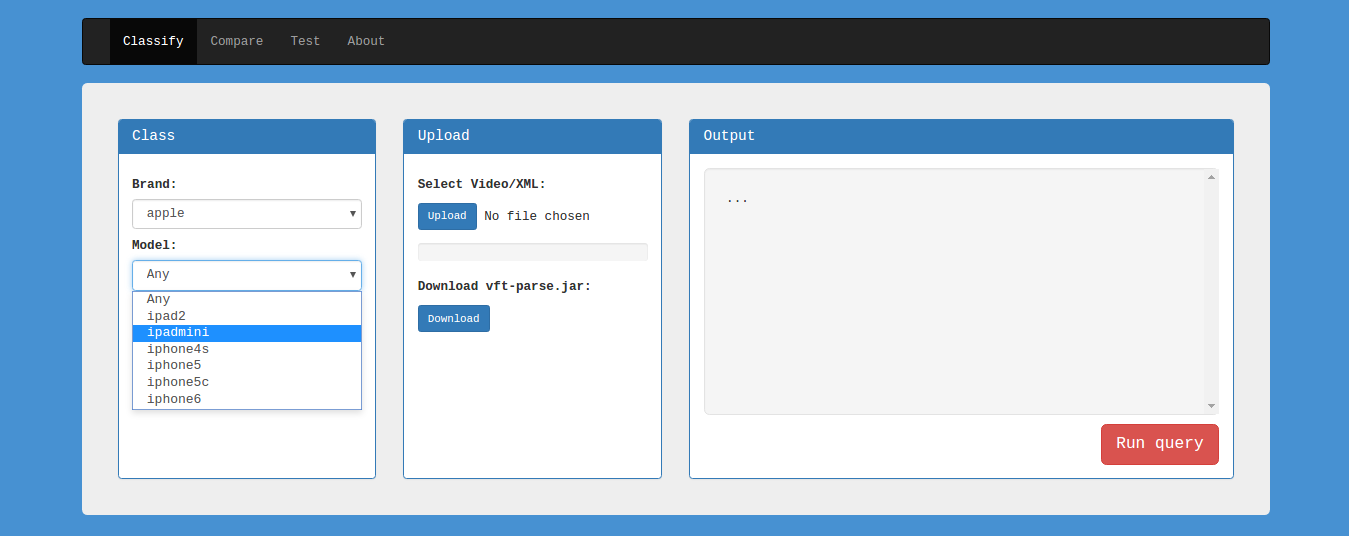
\includegraphics[width=1\textwidth]{classify}
  \caption{The user can select the class to test for the \emph{Classify} feature.}\label{fig:classify}
\end{figure}

It can work in two different ways. If the user explicitly selects a class (a brand, a brand, and a model, or a brand a model and an operating system), the method will execute in manual mode. If the user leaves the default values \emph{Any} from each selection, the method will run in automatic mode.

The manual mode is used when the user already has an assumption about the query video source device and wants to assess its correctness. Choosing a particular class is equal to asking a binary question: does the query video belongs to this selected class? The application will proceed to split the ground truth accordingly and will compute and return the likelihood for the query video regarding the selected device class.

The automatic mode is typically used when no assumption is made about the query video origin. Instead one binary problem, we pose as many binary problems as there are classes of devices in our ground truth dataset of videos. For each class, the likelihood will be computed and then sorted with regards to all other. The outputted result, as shown in \ref{fig:classify-output}, will be a list of classes sorted by likelihood in decreasing order.

\begin{figure}
  \centering
  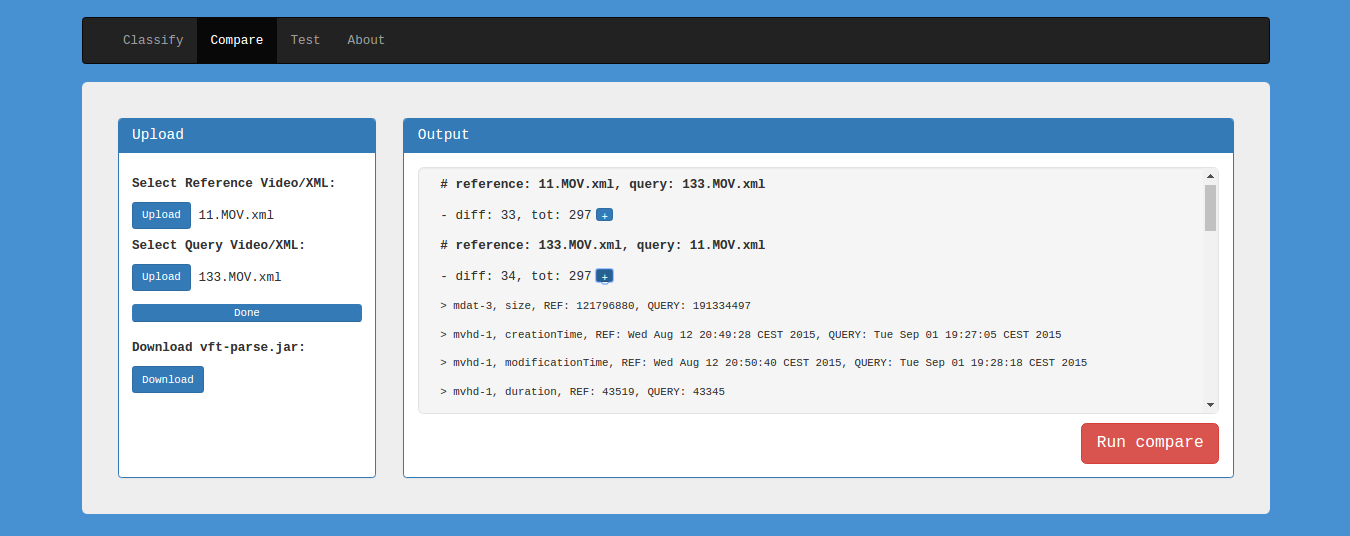
\includegraphics[width=1\textwidth]{classify-output}
  \caption{For the automatic mode of \emph{Classify}, the results will be shown as a list of classes sorted in decreasing order of likelihood}\label{fig:classify-output}
\end{figure}

The \emph{Classify} feature also allow the user to upload and compute the likelihood for more than one query video at a time.

Particular attention must be reserved in how the ground truth is split once a class $C$ to test is chosen. In fact, we have found that the results can be significantly affected by the reference population, in our case the complementary class $\overline{C}$. This problem also affects other application of forensic analysis, mainly in Speaker Recognition. Thus, it is important to decide if the reference population must represent a sample of the entire population or a sample of the population that presents similar characteristics to the population of the class under examination. For our case, this question translates to choosing if the class $\overline{C}$ should contain a sample of all the videos in the ground truth that do not belong to the class $C$, or a sample of all videos in the ground truth that do not belong to the class $C$ but that are similar to the videos in class $C$.

We decide for the latter approach.
If a class is composed of brand, model, and operating system the complementary class $\overline{C}$ is chosen by taking the videos of the ground truth that have the same brand and model but a different operating system.
If a class is composed of brand and model, leaving the default value Any to the operating system field, the complement class $\overline{C}$ is chosen by taking the videos of the ground truth from the same brand but that have a different model.
Finally, if for a class is specified only the brand field, the complementary class $\overline{C}$ is composed by a sample of all the videos from the ground truth that are from a different brand. This case is the most general and equivalent to choosing a sample of the entire population as the reference.

\item[-] \emph{Compare}: this functionality allows the user to verify the integrity of a query video, exploiting the \emph{compare} feature of the \emph{Video Format Tool} application. The user must upload two videos, one representing the reference and the other the query for which the integrity must be assessed. Once the operation is concluded, in the Output box will be shown the results of the comparison by displaying the number of difference that the query videos have with regards to the reference video and vice-versa. It is also possible to show the atoms and the attributes for which the differences are found, as shown in \ref{fig:compare}.

\begin{figure}
  \centering
  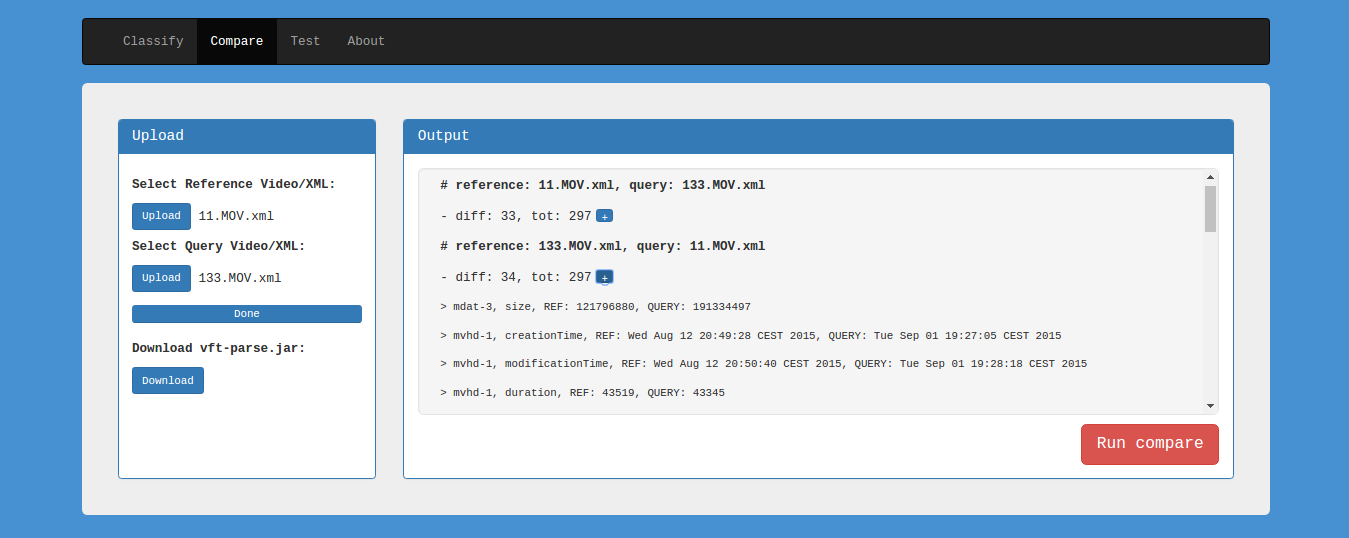
\includegraphics[width=1\textwidth]{compare}
  \caption{For the \emph{Compare}, it is also shown the atoms and the attributes for which the differences are found.}\label{fig:compare}
\end{figure}

\item[-] \emph{Test}: the \emph{Test} functionality is just an utility to iterate the \emph{Classify} over many videos without the need to manually upload each one. In fact, the query videos are stored in a table of the web application database along with information about their true class. The output results will be the same as for the \emph{Classify} but with the addition of statistics about the accuracy of the classification.

\end{itemize}

For both the \emph{Classify} and \emph{Compare} functionality, it is possible to upload a query video directly as a video file. However, since this is a web application, there could be some limitations in the upload speed of a user making the whole process slow. As mention previously it possible to upload the XML file representing a video file container as a query but, in general, a user might not possess the instrument to acquire such XML file. For this reason, we have also developed a simple Java \emph{Swing} GUI application that can be downloaded from the web application. This app allows the user to parse a video file into an XML file representing its file container, using the parse feature from the \emph{Video Format Tool}, as well as parsing an entire folder. In this way, due to the small size of a generic XML file, it is possible to execute a query seamlessly.